\documentclass{zjureport}
% =============================================
% Part 1 Edit the info
% =============================================

\newcommand{\major}{测控技术及仪器}
\newcommand{\name}{郑成琦}
\newcommand{\stuid}{3179801017}
\newcommand{\newdate}{2020-4-8}
\newcommand{\loc}{家}

\newcommand{\course}{EDA技术应用}
\newcommand{\tutor}{黄添添}
\newcommand{\grades}{None}
\newcommand{\newtitle}{四位计数器设计}
\newcommand{\exptype}{设计与编码实验}
\newcommand{\group}{None}

% =============================================
% Part 1 Main document
% =============================================
\begin{document}
\thispagestyle{empty}
\begin{figure}[h]
  \begin{minipage}{0.6\linewidth}
    \centerline{\includegraphics[width=\linewidth]{head.jpg}}
  \end{minipage}
  \hfill
  \begin{minipage}{.4\linewidth}
    \raggedleft
    \begin{tabular*}{.8\linewidth}{ll}
      专业: & \underline\major   \\
      姓名: & \underline\name    \\
      学号: & \underline\stuid   \\
      日期: & \underline\newdate \\
      地点: & \underline\loc
    \end{tabular*}
  \end{minipage}
\end{figure}

\begin{table}[!htbp]
  \centering
  \begin{tabular*}{\linewidth}{llllll}
    课程名称: & \underline\course   & 指导老师: & \underline\tutor   & 成绩:       &  \underline\grades \\
    实验名称: & \underline\newtitle & 实验类型: & \underline\exptype & 同组学生姓名:& \underline\group
  \end{tabular*}
\end{table}

% =============================================
% Part 2 Main document
% =============================================

\section{实验目的和要求}
1、了解Quartus II开发环境,熟悉Verilog语言基本语法

2、实现4位计数器选择功能
\section{实验内容和步骤}

  \subsection{实验内容}
	根据所给的手册《My First FPGA》进行实验操作。最后在上述基础上加入计数选择功能。
  \subsection{实验步骤}
	\begin{clause}
		\item 计数器的HDL语言编写
		\item PLL模块调用
		\item Multiplexer模块调用
		\item 进行编译
		\item 进行时序仿真
	\end{clause}
\section{主要仪器设备}
  计算机,Quartus

\section{操作方法和实验步骤}
  \subsection{计数器HDL语言编写}
    \lstinputlisting[language=Verilog]{FPGA_EDA_one/simple_counter.v}
  \subsection{PLL模块调用}
    (因为软件原因,模块显示在我的电脑是挤在一起十分混乱)
    \begin{clause}
      \item 模块图片
      \begin{center}
        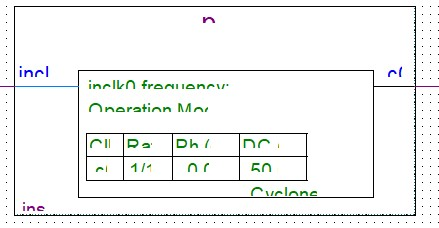
\includegraphics[width=0.6\linewidth]{PLL.jpg}
      \end{center}
      \item 模块连线 
      \begin{center}
        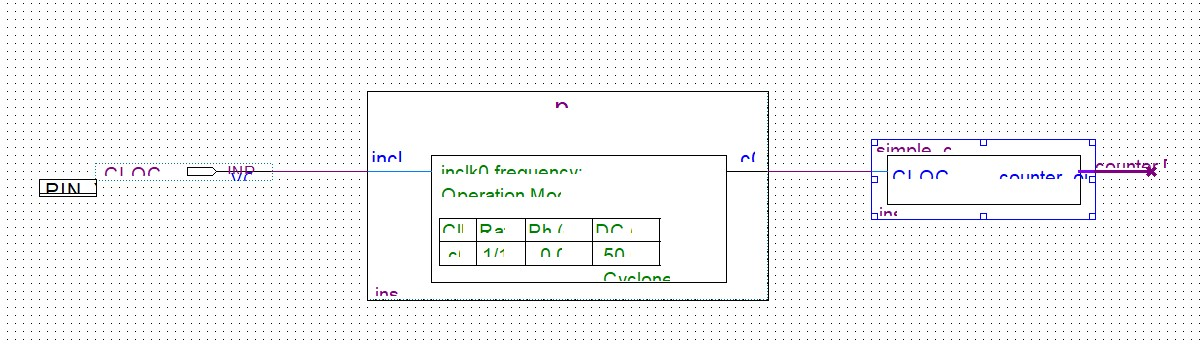
\includegraphics[width=0.6\linewidth]{figures/Link_1.jpg}
        \\PLL的输出作为计数器的输入来作为主要的计数速度控制手段。
      \end{center}
    \end{clause}
  \subsection{Multiplexer模块调用}
    同样也是根据参考教程完成,该部分的模块调用,这部分调用的目的主要是实现输出可以通过LED显示。

    (因为软件的问题,显示仍然很混乱)
    \begin{center}
      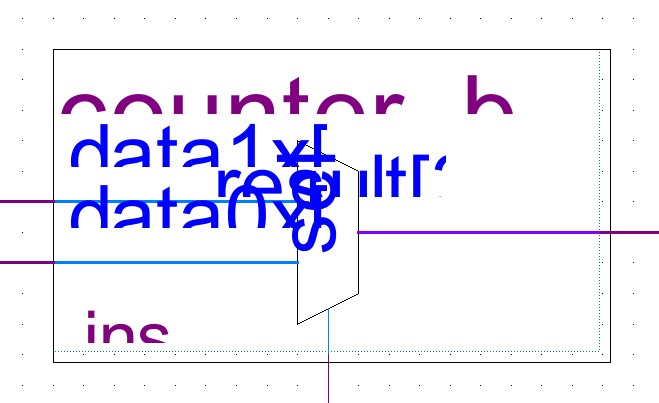
\includegraphics[width=0.6\linewidth]{figures/Mux.jpg}
    \end{center}
    
    这个模块有三个输入其中两个分别是计数器模块的输出,根据手册这个模块的分别引入了计数器的输出的不同的四位数部分,
    这也是输出计数的不同速度的原因;还有一个输入用于选择具体采用哪一个输入,一个输出用于连接FPGA的LED模块。
  \subsection{编译}
    当按下“Start Compilation”Quartus开始运行仿真。仿真完全通过。
    \begin{center}
      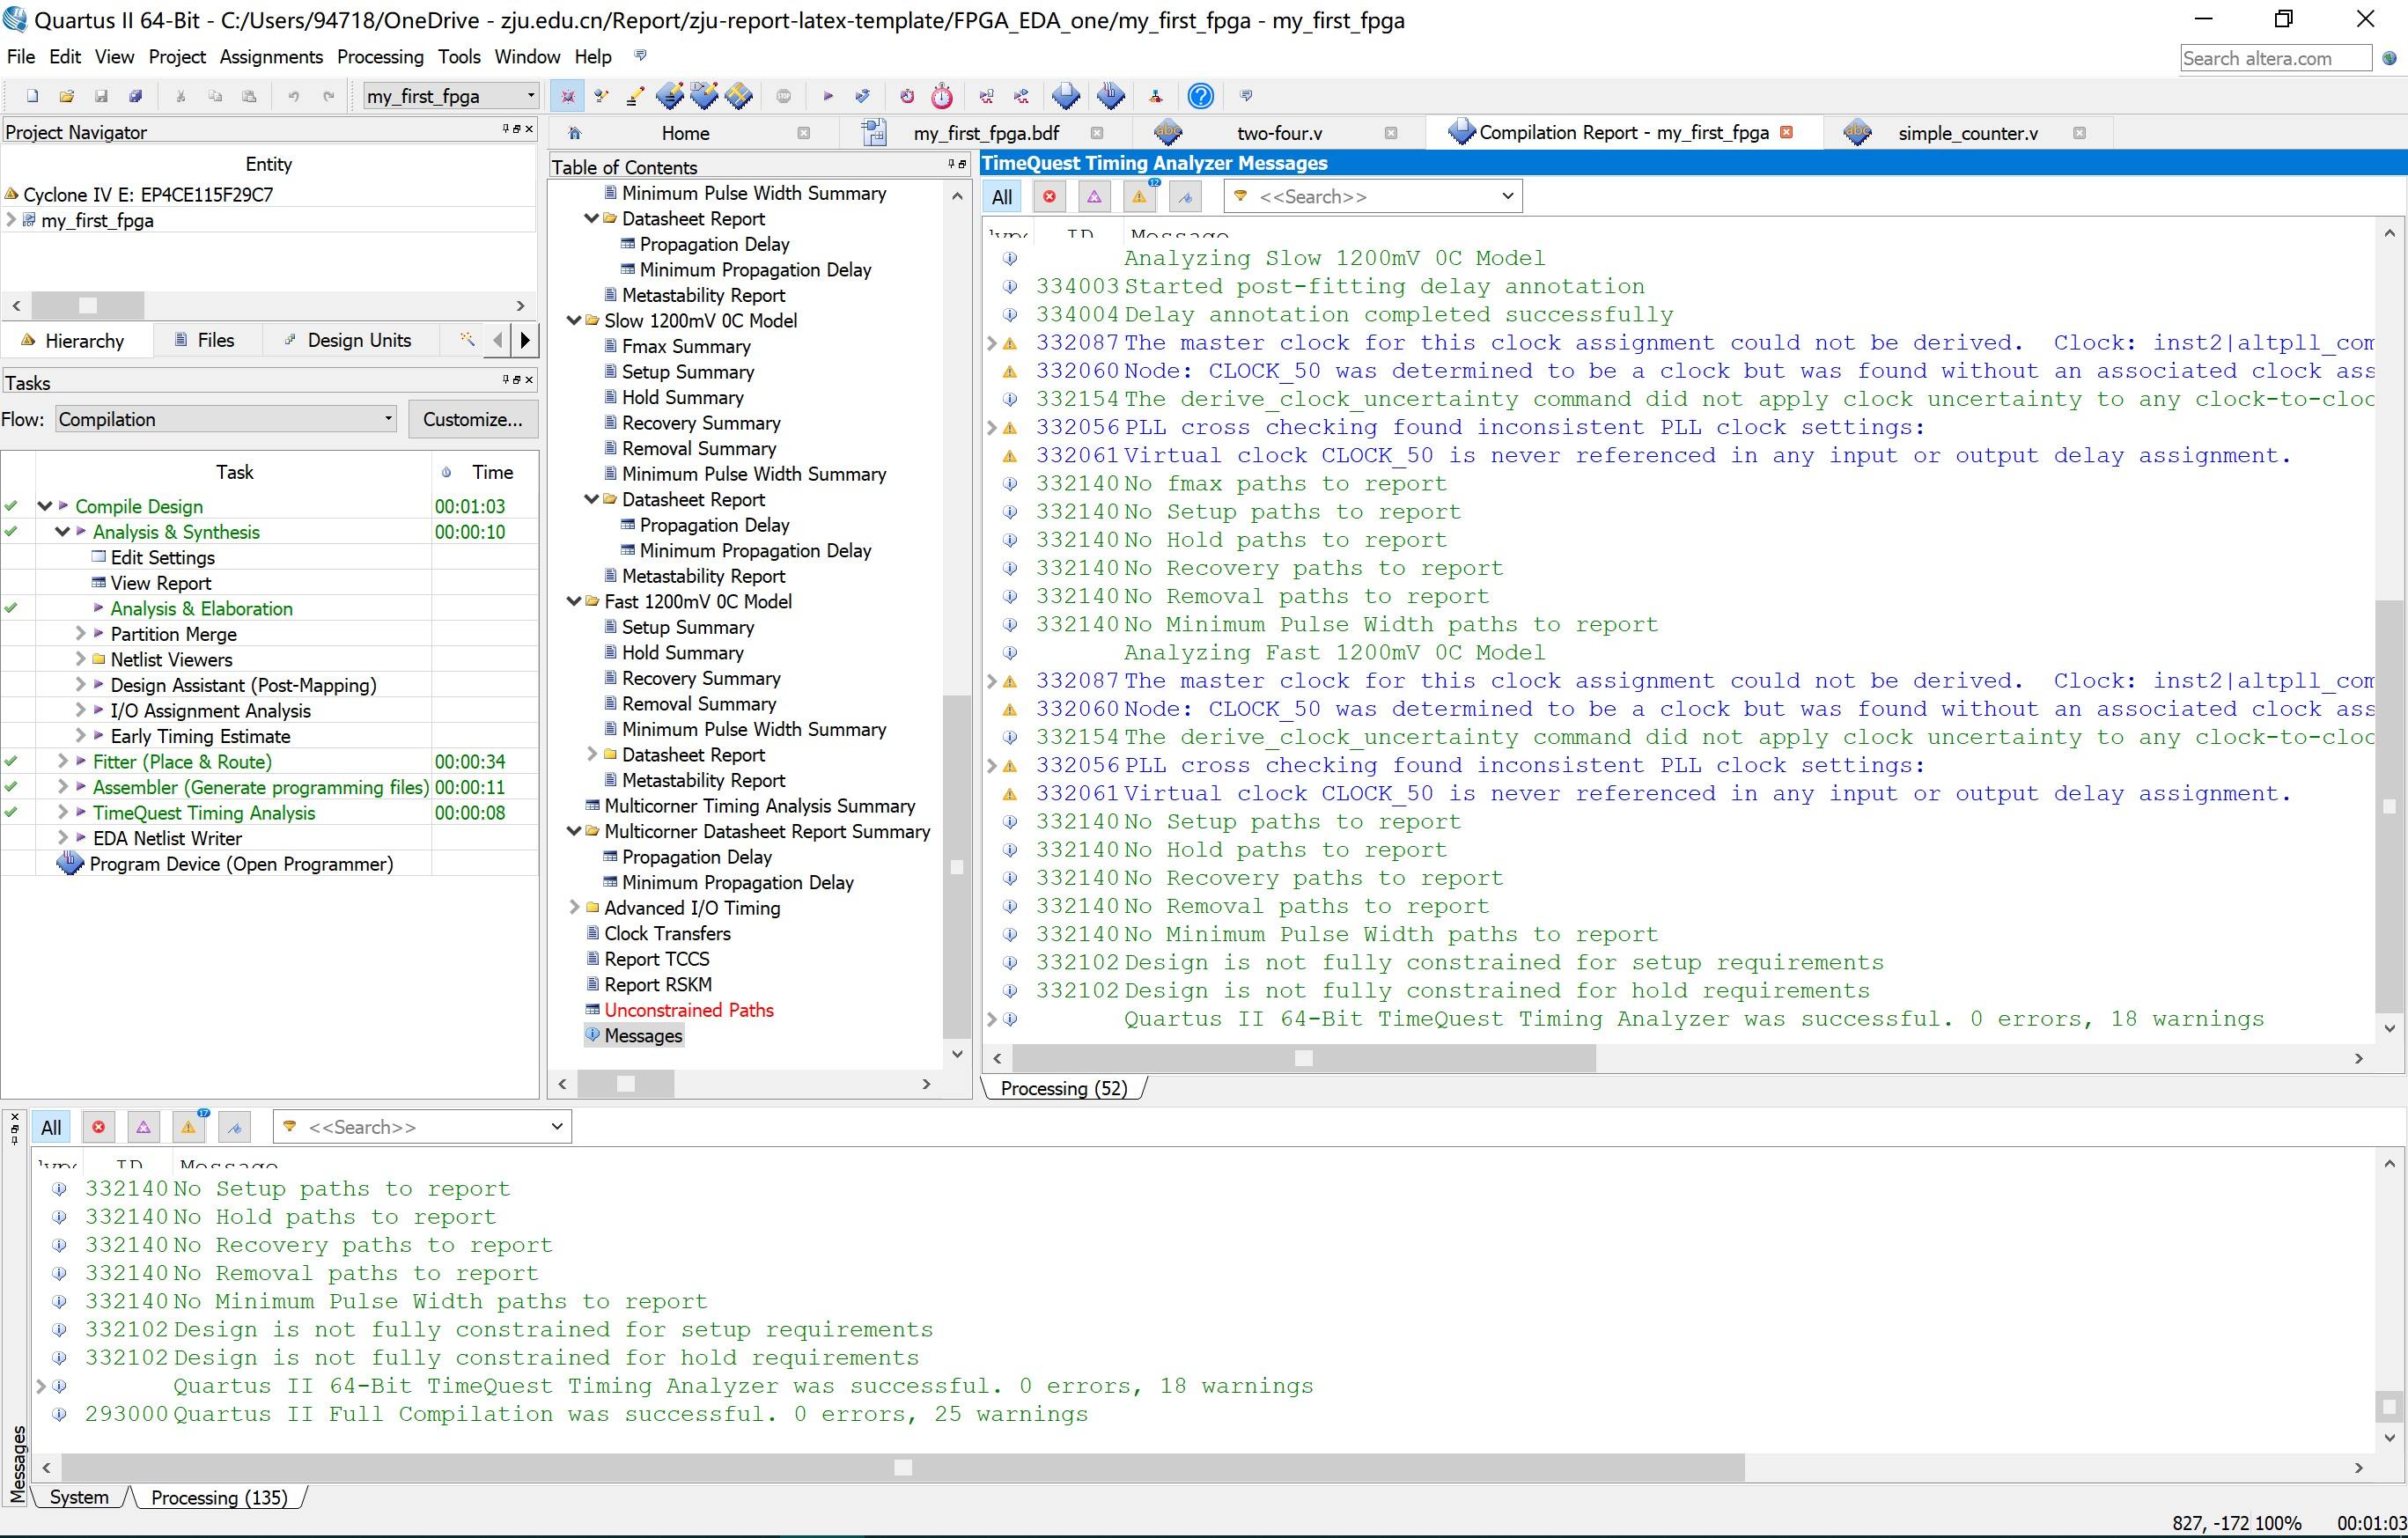
\includegraphics[width=0.6\linewidth]{figures/Compilation.jpg}
    \end{center}
\section{实验数据记录和处理}
  \subsection{系统的整体图}
  (软件原因,图形展示不完整)
  \begin{center}
    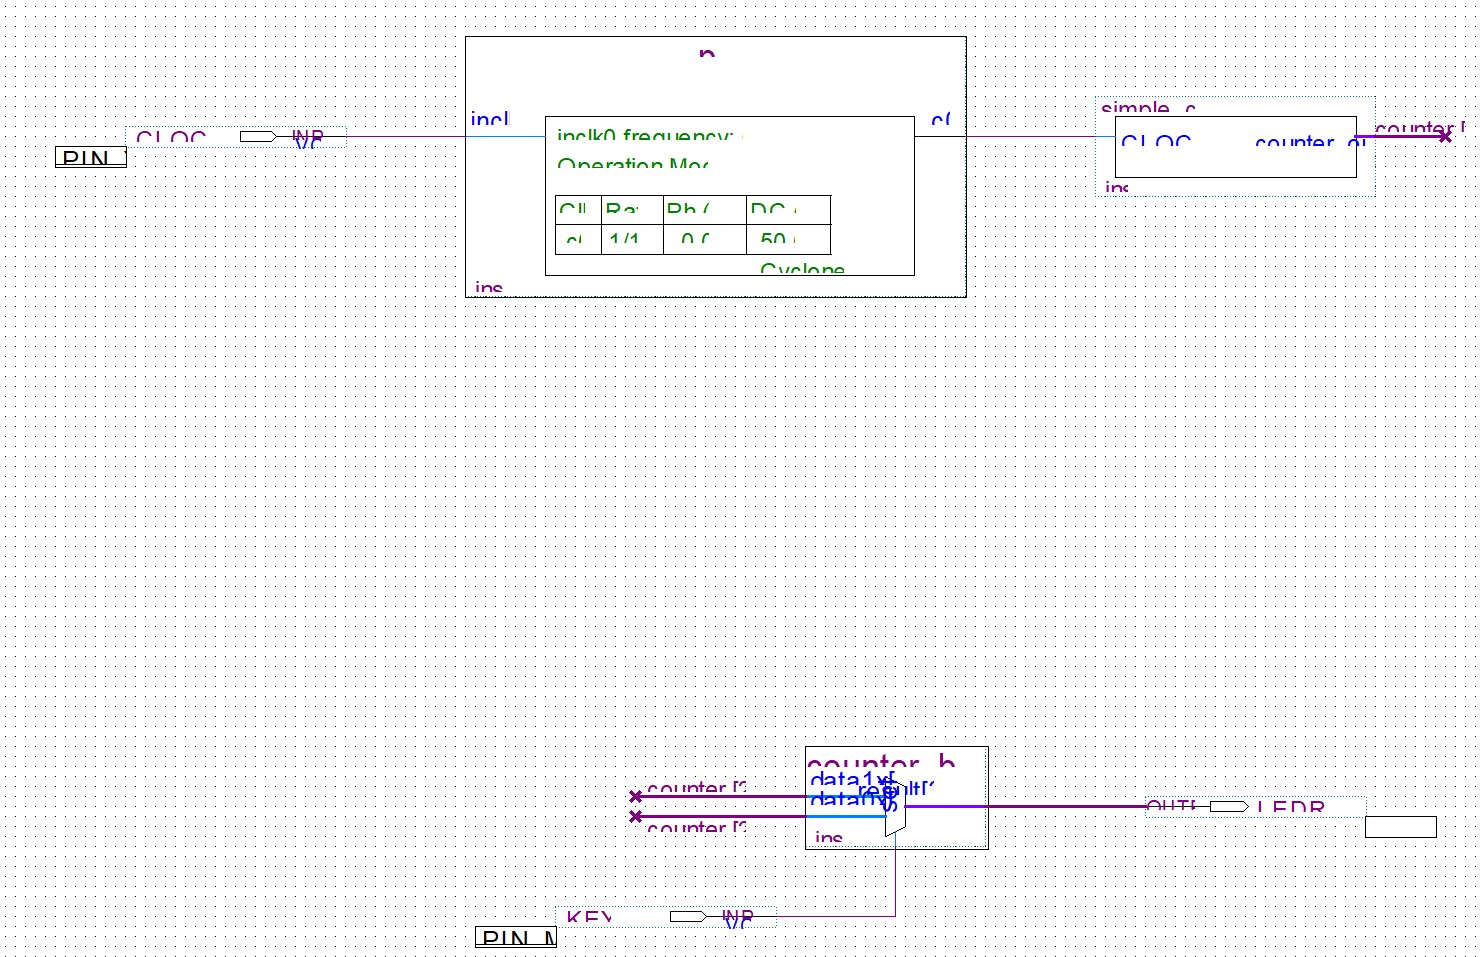
\includegraphics[width=0.6\linewidth]{figures/total.jpg}
  \end{center}
  \subsection{编译测试结果}
  预计结果是通过。确实通过,但是在此之前有很多问题,比如说:
  \begin{clause}
    \item 软件破解不完全,导致最后的仿真失败没有产品license权限。
    \item 引脚属性不对应,导致连线报错。
    \item 对同一个引脚有两个输入,导致报错。
  \end{clause}
  \subsection{时域图分析失败}
  这部分,搞了很久,始终不知道为什么会出错。
\section{实验结果与分析}
因为时序图出错,同时没有FPGA的开发板所以实验结果和分析这部分内容以后再补充。

在此说明一下,实现不同速度的计数的原理,以补充分析的内容。

这里的LED输出有两种模式,分别对应Multiplexer的两个不同的输入。它的两个不同的输入分别是来自计数器的输出的不同部分
,分别是来自输出的"21-24"和输出的“26-23”位。直观来说,前者比后者计数更快,因为其仅仅需要$2^{21} $次CLOCK上升沿输入信号,就可以加一。
而后者需要$2^{23}$次CLOCK上升沿输入信号才可以加一。

通过对KEY进行赋值,可以让输出在两种速度中切换。
\end{document}
